%!TeX encoding=utf8
%%%%%%%%%%%%%%%%%%%%%%%%%%%%%%%%%%%%%%%%%%%%%%%%%%%%%%%%%%%%%%%%%%%%%%%%%%%%%%%%
% Vorlage für mit LaTeX formatierte Versuchsberichte im Physikpraktium
%%%%%%%%%%%%%%%%%%%%%%%%%%%%%%%%%%%%%%%%%%%%%%%%%%%%%%%%%%%%%%%%%%%%%%%%%%%%%%%%
% Diese Datei steht unter der Lizenz CC0 1.0 . Sie darf kopiert, verändert
% und weitergegeben werden. Zu den Details siehe
% https://creativecommons.org/publicdomain/zero/1.0/deed.en
%%%%%%%%%%%%%%%%%%%%%%%%%%%%%%%%%%%%%%%%%%%%%%%%%%%%%%%%%%%%%%%%%%%%%%%%%%%%%%%%

\documentclass[ngerman]{scrartcl}

% Passen Sie hier *Author1*, *Author2* und *Grp.-Nr.* an.
\newcommand{\authA}{*Author1*}
\newcommand{\authB}{*Author2*}
\newcommand{\grpnr}{*Grp.-Nr.*}

%%%%%%%%%%%%%%%%%%%%%%%%%%%%%%%%%%%%%%%%%%%%%%%%%%%%%%%%%%%%%%%%%%%%%%%%%%%%%%%%
% Vorspann für mit LaTeX formatierte Versuchsberichte im Physikpraktium
%%%%%%%%%%%%%%%%%%%%%%%%%%%%%%%%%%%%%%%%%%%%%%%%%%%%%%%%%%%%%%%%%%%%%%%%%%%%%%%%
% Diese Datei steht unter der Lizenz CC0 1.0 . Sie darf kopiert, verändert
% und weitergegeben werden. Zu den Details siehe
% https://creativecommons.org/publicdomain/zero/1.0/deed.en
%%%%%%%%%%%%%%%%%%%%%%%%%%%%%%%%%%%%%%%%%%%%%%%%%%%%%%%%%%%%%%%%%%%%%%%%%%%%%%%%


% Optionen für die Dokumentenklasse scartcl von KOMAscript.
\KOMAoptions{
	DIV=11,
	BCOR=0mm,
	paper=a4,
	fontsize=12pt,
	parskip=half,
	twoside=false,
	titlepage=false
}

% Papierformat: DIN-A4, mit wenig Rand
\usepackage[
	a4paper,
	left=20mm,
	right=20mm,
	top=23mm,
	bottom=15mm,
	includefoot,
	footskip=8mm
	]{geometry}

% Zeilenabstand, andere Werte: onehalfspacing, doublespacing
\usepackage[singlespacing]{setspace}

% Definition der Kopf- und Fußzeile
\usepackage[headsepline,automark]{scrlayer-scrpage}
\clearpairofpagestyles
\setlength{\headheight}{2.5\baselineskip}
\setlength{\footheight}{1\baselineskip}
\ihead[]{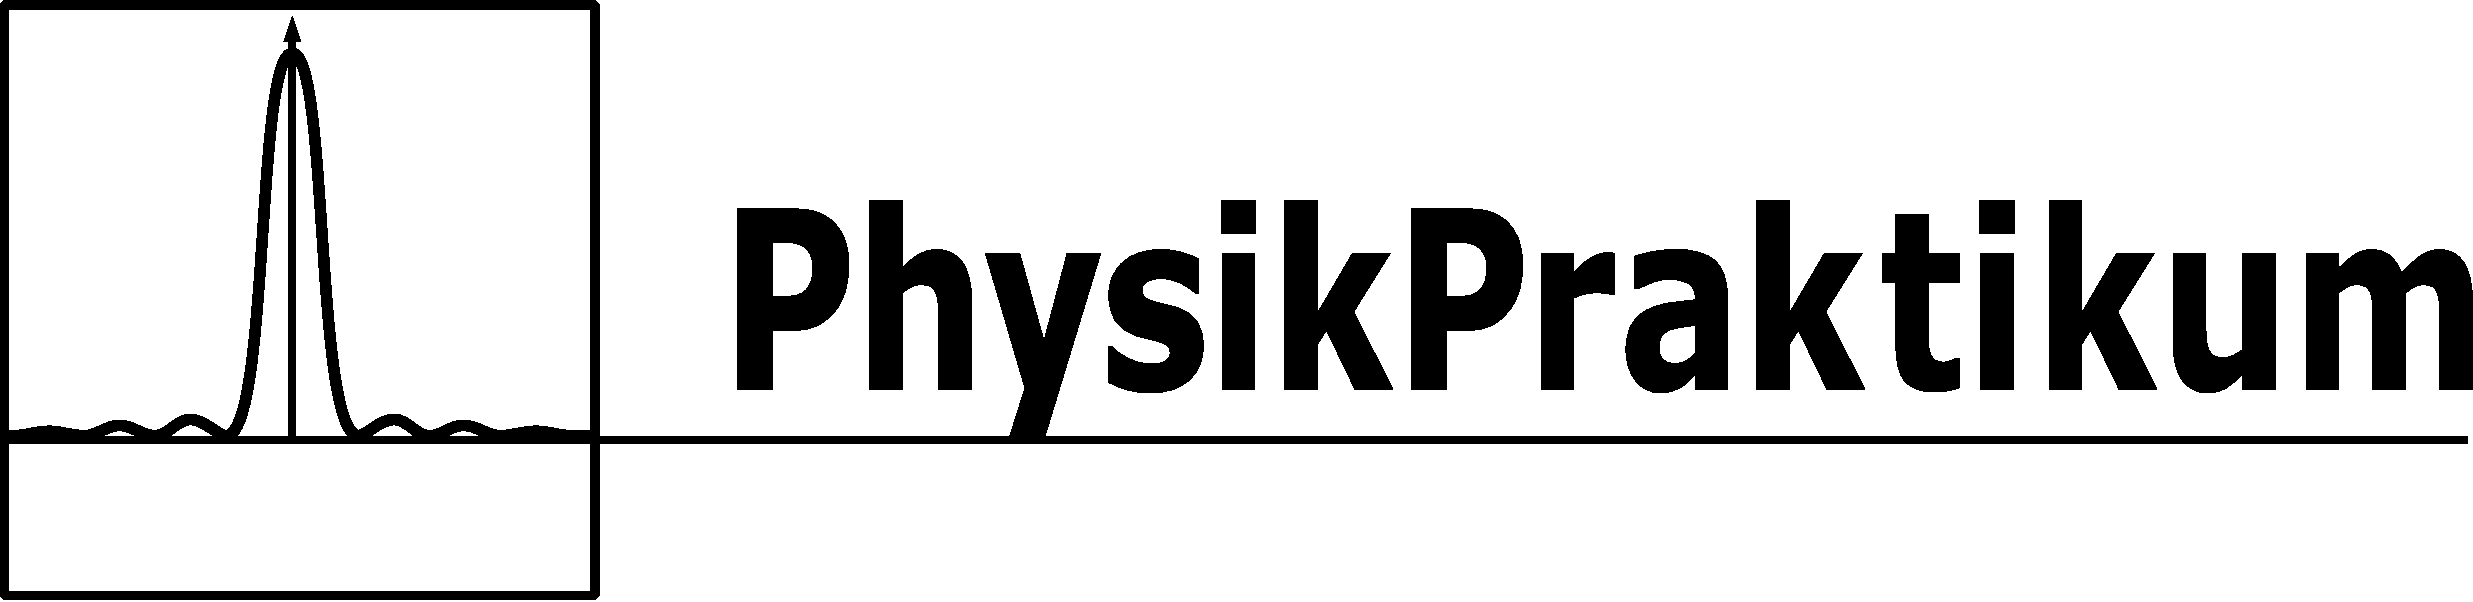
\includegraphics[width=4cm]{Images/ap-logo_bw.pdf}}
\chead[]{\authA \\ \authB}
\ohead[]{Datum: \today \\ Gruppe:~\grpnr}
\ofoot[]{\pagemark}

%---Language and umlauts
\usepackage[utf8]{inputenc}       % UTF-8 Kodierung - ä, ö, ü, ß direkt eingeben
\usepackage[ngerman]{babel}                      % Neue deutsche Rechtschreibung
\usepackage[expansion=true, protrusion=true]{microtype} % Bessere Silbentrennung

% Formelsatz
\usepackage{amsmath}		% Mathematik-Umgebungen - z.B. align
\usepackage{amsthm}		% Umgebung "theorem"
\usepackage{amsfonts}	% Schriften
\usepackage{amssymb}		% Symbole
\usepackage{upgreek}		% Griechische Sonderzeichen z.B. \upmu

% Einheiten
\usepackage{siunitx}
\sisetup{
	locale = DE,
	separate-uncertainty,
	range-units = brackets,
	list-units = single,
	per-mode=fraction
}

% Bilder und Tabellen
\usepackage{graphicx}			% Bilder als PDF einbinden
\usepackage{epstopdf}			% Bilder im EPS-Format
\usepackage{caption}				% Unterschriften für Bilder und Tapellen
\usepackage{booktabs}			% Zusätzliche Schönheitslinien für Tabellen
\usepackage{multirow}			% Mehrere Felder in einer Tabelle zusammenfassen
\usepackage[table]{xcolor}		% Für farbig unterlegte Tabellenzeilen
  \definecolor{lightgray}{gray}{0.9}
  \rowcolors{1}{}{lightgray}	% jede zweite Zeile in einer Tabelle leicht grau


% Positionierung von Bildern und Tabellen
\usepackage{float}				% Option 'H', also "hier-egal-wie-das-aussieht"
\usepackage[section]{placeins}	% Platzierung spätestens am Ende eines Kapitels
\renewcommand{\floatpagefraction}{.75}	% standard: .5
\renewcommand{\textfraction}{.1}			% standard: .2
\renewcommand{\topfraction}{.8}			% standard: .7
\renewcommand{\bottomfraction}{.5}		% standard: .3
\setcounter{topnumber}{3}				% standard: 2
\setcounter{bottomnumber}{2}				% standard: 1
\setcounter{totalnumber}{5}				% standard: 3

\usepackage{caption}
\captionsetup[figure]{name=Abbildung,format=plain}
\captionsetup[table]{name=Tabelle,format=plain}

\usepackage{copyrightbox}		% Nachweis der Bildquelle

% Schrift für die Bildquelle
\makeatletter
\renewcommand{\CRB@setcopyrightfont}{%
\usefont{T1}{cmr}{m}{n}\fontsize{10}{10}\selectfont }
\makeatother


% Hyperlinks
\usepackage{hyperref}
\hypersetup{
	colorlinks=true,
	breaklinks=true,
	citecolor=darkgray,
	linkcolor=darkgray,
	menucolor=red,
	urlcolor=cyan,
	bookmarksopen=false,
	bookmarksopenlevel=0,
	plainpages=false,			% zur korrekten Erstellung der Bookmarks
	hypertexnames=false			% zur korrekten Erstellung der Bookmarks
}

\usepackage{pdfpages} 		% Einfügen von Vollseiten-PDFs (z.B. das Deckblatt)
\pdfminorversion=7			% Das Deckblatt-Formular ist ein PDF, version 1.7
\usepackage{csquotes}		% Zitate

% Literaturverzeichnis
\usepackage[style=alphabetic,sorting=ynt,backend=biber]{biblatex}

% Eine Abkürzung, die Computerbefehle im Fließtext mit einer Mono-Schrift setzt
% (funktioniert leider nicht für Backslash \ . Da hilft dann der Befehl \verb )
\providecommand*{\code}[1]{{\texttt{#1}}}



% Latex-Vorspann für das Deckblatt des Physikpraktiums in Hannover
%%%%%%%%%%%%%%%%%%%%%%%%%%%%%%%%%%%%%%%%%%%%%%%%%%%%%%%%%%%%%%%%%%%%%%%%%%%%%%%%
% Diese Datei steht unter der Lizenz CC-BY-SA 4.0 . Sie darf kopiert, verändert
% und weitergegeben werden. Dabei müssen die Urheber genannt werden und die
% Lizenz beibehalten bleiben. Zu den Details siehe
% https://creativecommons.org/licenses/by-sa/4.0/
%%%%%%%%%%%%%%%%%%%%%%%%%%%%%%%%%%%%%%%%%%%%%%%%%%%%%%%%%%%%%%%%%%%%%%%%%%%%%%%%
% Autoren: Kim Weber, Kai-Martin Knaak, beide Leibniz-Universität Hannover
%%%%%%%%%%%%%%%%%%%%%%%%%%%%%%%%%%%%%%%%%%%%%%%%%%%%%%%%%%%%%%%%%%%%%%%%%%%%%%%%

\usepackage{afterpage}	% die Seitennummerierung nach dem Deckblatt beginnen

% für die Ankreuz-Felder
\newcounter{irow}
\setcounter{irow}{0}
\usepackage{tcolorbox}
\newcommand {\janein}{\llap{Ja \: Nein \, n.a. \hspace*{0.5mm}}}
\newcommand {\kaestchen}{\hfill{\llap{
			\CheckBox[name=\theirow*3,charsize=10pt,width=8pt,height=8pt]{}
			$\quad$ \CheckBox[name=\theirow*3+1,charsize=10pt,width=8pt,height=8pt]{}
			$\quad$ \CheckBox[name=\theirow*3+2,charsize=10pt,width=8pt,height=8pt]{}}
			}\hspace*{3mm}
			\stepcounter{irow}}

\usepackage{tikz}		% um den Strich unter dem Stempelfeld zu malen



\addbibresource{Literatur.bib}


\begin{document}

% Latex-Formular für das Deckblatt des Physikpraktiums in Hannover
%%%%%%%%%%%%%%%%%%%%%%%%%%%%%%%%%%%%%%%%%%%%%%%%%%%%%%%%%%%%%%%%%%%%%%%%%%%%%%%%
% Diese Datei steht unter der Lizenz CC-BY-SA 4.0 . Sie darf kopiert, verändert
% und weitergegeben werden. Dabei müssen die Urheber genannt werden und die
% Lizenz beibehalten bleiben. Zu den Details siehe
% https://creativecommons.org/licenses/by-sa/4.0/
%%%%%%%%%%%%%%%%%%%%%%%%%%%%%%%%%%%%%%%%%%%%%%%%%%%%%%%%%%%%%%%%%%%%%%%%%%%%%%%%
% Autoren: Kim Weber, Kai-Martin Knaak, beide Leibniz-Universität Hannover
%%%%%%%%%%%%%%%%%%%%%%%%%%%%%%%%%%%%%%%%%%%%%%%%%%%%%%%%%%%%%%%%%%%%%%%%%%%%%%%%

\thispagestyle{empty}

\afterpage{%
\newgeometry{left=10mm,right=10mm,top=5mm,bottom=5mm}

\begin{Form}
	{\raisebox{-0.35\height}{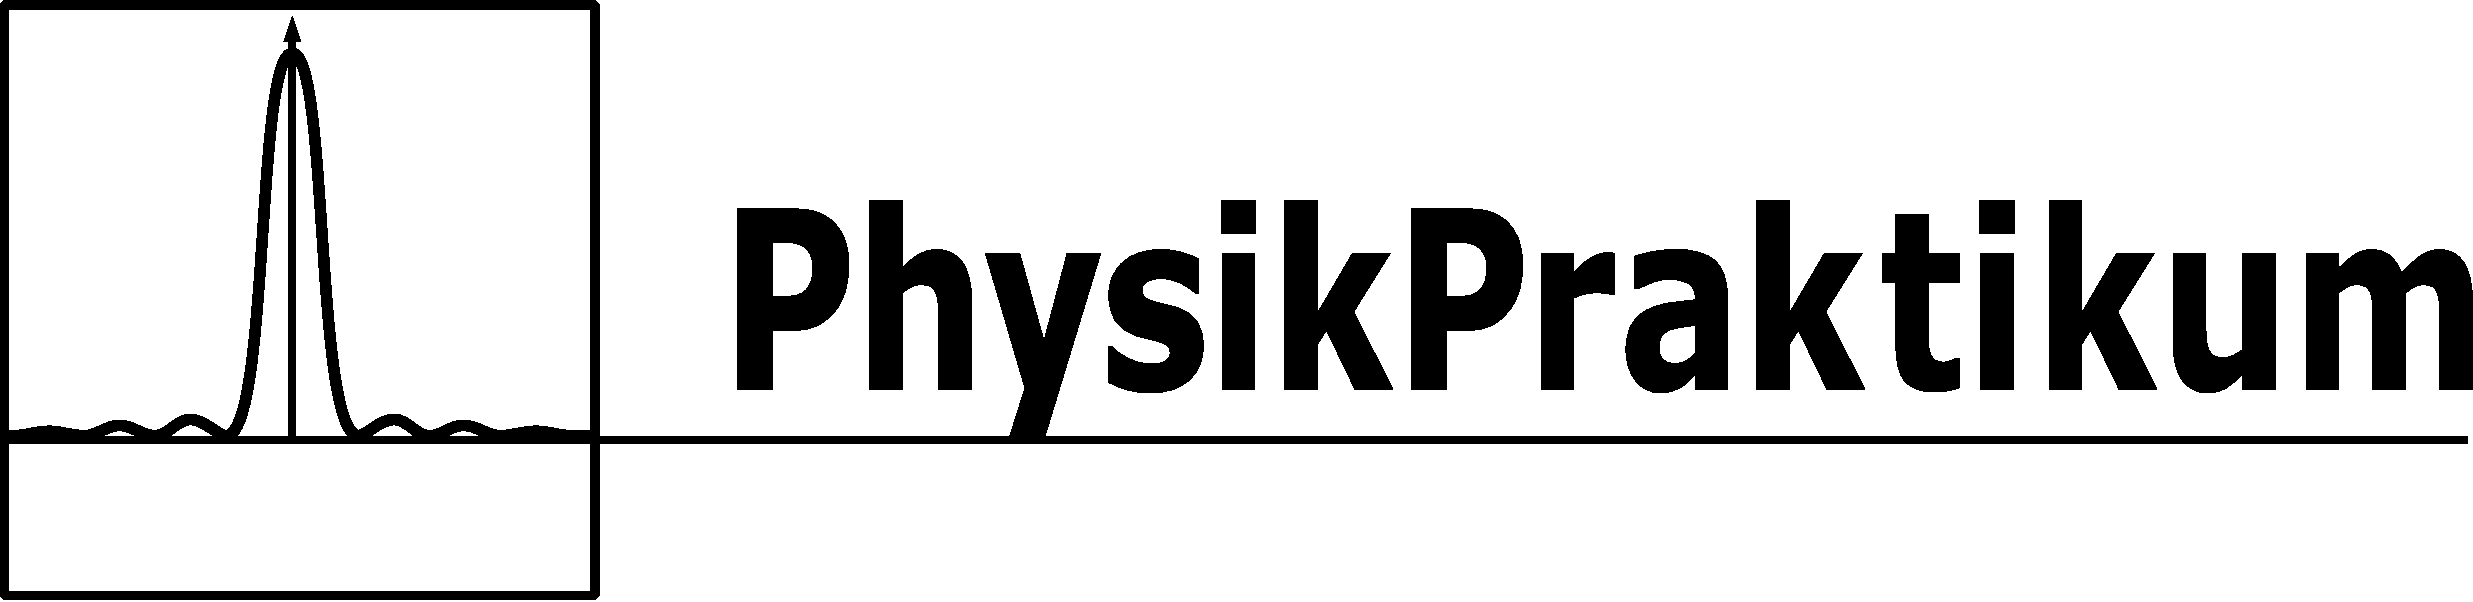
\includegraphics[width=0.4\textwidth]{Images/ap-logo_bw.pdf}}
	\hfill \Large Bericht zum Versuch: \underline{\TextField[name=Versuchsnummer,width=0.25 \textwidth,height=18pt,charsize=14pt,align=1]{}}}

\begin{tcolorbox}[coltitle=black,colbacktitle=black!10!white
		,title={Angaben zum Experiment}
		,sidebyside, sidebyside gap=1mm, righthand width=6cm, lower separated=false
		,toptitle=1mm
		,width=\linewidth-3mm]
	\begin{tabular}{lc}
		Name: & \underline{\TextField[name=Name, width=0.5 \textwidth,height=15pt,charsize=12pt]{}}\\
		Gruppennummer: & \underline{\TextField[name=GPNR, width=0.5 \textwidth,height=15pt,charsize=12pt]{}}\\
		Versuchsleiter:&\underline{\TextField[name=VSL,width=0.5 \textwidth,height=15pt,charsize=12pt]{}}\\
		Datum des Versuchs: & \underline{\TextField[name=VD,width=0.5 \linewidth,height=15pt,charsize=12pt]{}} \\
		Datum der Abgabe: & \underline{\TextField[name=VA,width=0.5 \textwidth,height=15pt,charsize=12pt]{}} \\
	\end{tabular}
	\tcblower
	\TextField[name=PT,width=1.0 \textwidth,height=80pt,charsize=64pt,align=1]{}
	\begin{tikzpicture}
	\draw (0,0) -- node[below]{\footnotesize Stempel/Tutor-Unterschrift/Punkte}++(6,0);
	\end{tikzpicture}
\end{tcolorbox}

\begin{tcolorbox}[coltitle=black, colbacktitle=black!10!white
		,title={Allgemeines \hfill \janein }
		,toptitle=1mm
		,width=\linewidth-3mm]
	\begin{itemize}
		\setlength\itemsep{0em}
		\item{Abgabe des Berichts erfolgte pünktlich \kaestchen}
		\item{Äußere Form des Berichts ist angemessen \kaestchen}
		\item{Messdaten liegen dem Bericht bei \kaestchen}
		\item{Jede gedruckte Seite enthält Namen und Gruppennummer \kaestchen}
		\item{Es war keine Nachbesserung erforderlich \kaestchen}
	\end{itemize}
\end{tcolorbox}

\begin{tcolorbox}[coltitle=black, colbacktitle=black!10!white
		,title={Strukturierung und Dokumentation \hfill \janein }
		,toptitle=1mm
		,width=\linewidth-3mm]
	\begin{itemize}
		\setlength\itemsep{0em}
		\item{Der Bericht ist für sich stehend verständlich \hfill \kaestchen}
		\item{Rechenwege zur Ermittlung des Ergebnisses sind nachvollziehbar\hfill \kaestchen}
		\item{Unsicherheiten wurden richtig ermittelt (Fehlerfortpflanzung)\hfill \kaestchen}
		\item{Alle quantitativen Ergebnisse enthalten Angaben zur Messunsicherheit\hfill \kaestchen}
		\item{Messunsicherheiten und Ergebnisse werden diskutiert\hfill \kaestchen}
	\end{itemize}

\end{tcolorbox}
	\begin{tcolorbox}[coltitle=black, colbacktitle=black!10!white
		,title={Graphische Darstellung \hfill \janein }
		,toptitle=1mm
		,width=\linewidth-3mm]
	\begin{itemize}
		\setlength\itemsep{0em}
		\item{Bildunterschriften sind aussagekräftig \hfill \kaestchen}
		\item{Achsen sind vollständig bezeichnet und sinnvoll skaliert \hfill \kaestchen}
		\item{Messunsicherheiten sind mit Fehlerbalken dargestellt \hfill \kaestchen}
		\item{Bei Fit-Analysen sind alle relevanten Parameter angegeben \hfill \kaestchen}
		\item{Bei übernommenen Bildern ist die Quelle angegeben \hfill \kaestchen}
	\end{itemize}
\end{tcolorbox}

\begin{tcolorbox}[coltitle=black, colbacktitle=black!10!white
		,title={Anmerkungen}
		,sidebyside, sidebyside gap=1mm
		,toptitle=1mm
		,lower separated=false
		,width=\linewidth-3mm]
	\TextField[name=FB,multiline,width=\textwidth,height=48mm]{}%
	\tcblower
	\TextField[name=FB,multiline,width=\textwidth,height=48mm]{}%
\end{tcolorbox}

\scriptsize Deckblatt Physikpraktikum, Version 3.1 / \today
\hfill Kim Weber, Kai-Martin Knaak, Lizenz: {\href{https://creativecommons.org/licenses/by-sa/4.0/}{CC BY-SA 4.0}}

\end{Form}

\restoregeometry
}

	% Das Praktikumsdeckblatt einbinden

\shorthandoff{"}			% Anführungszeichen nicht als Befehl interpretieren

\subject{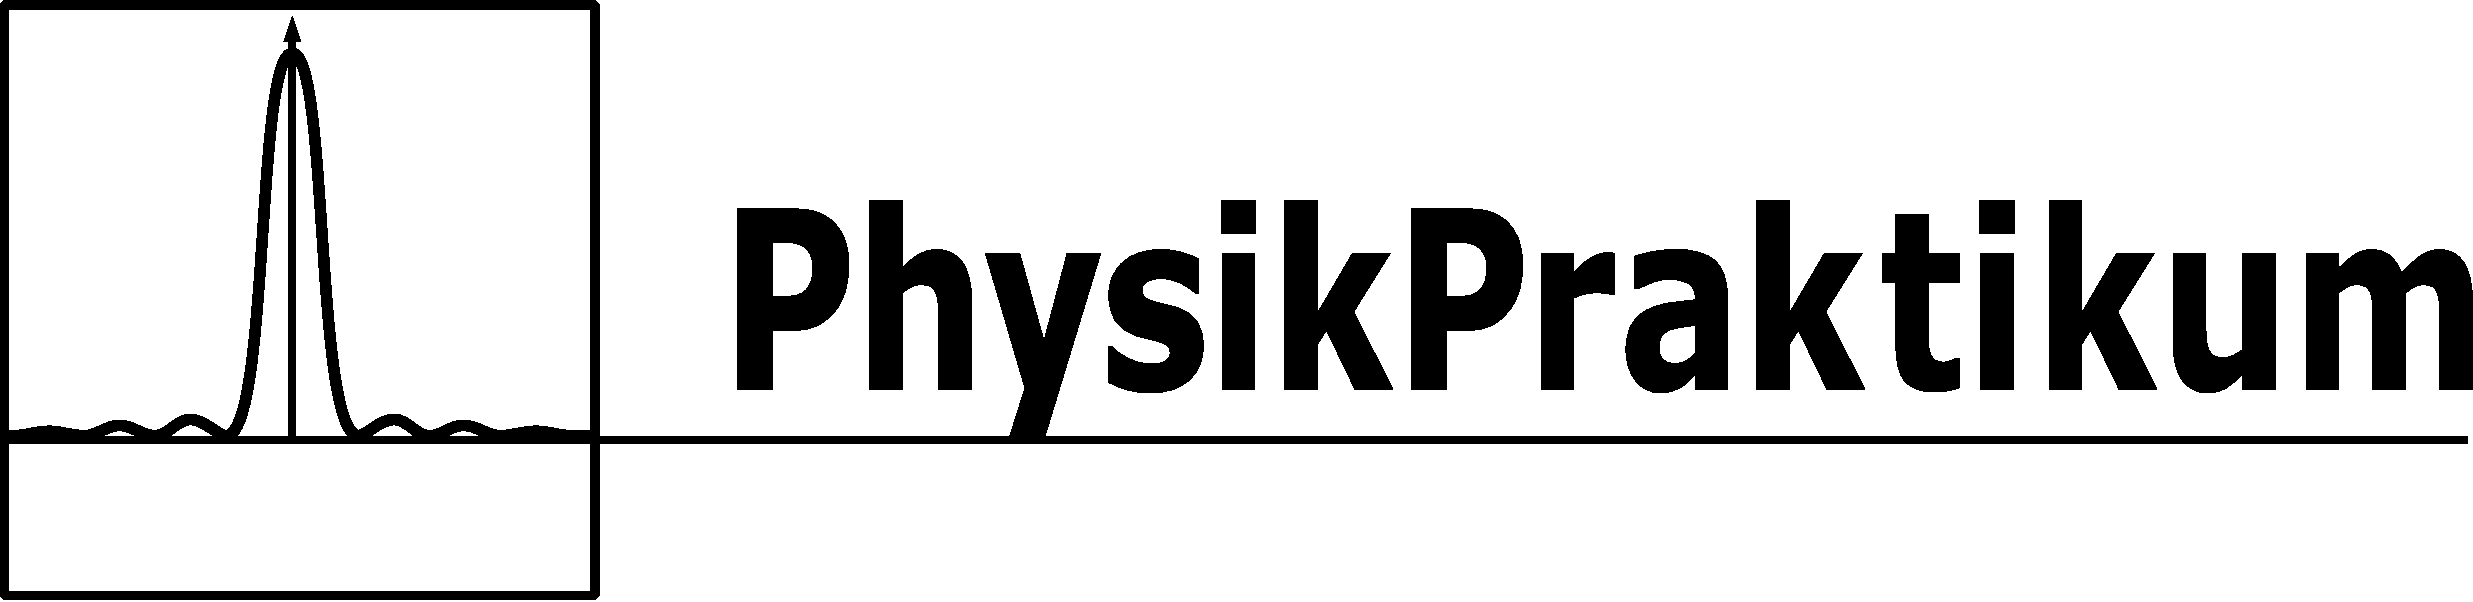
\includegraphics[width=8cm]{Images/ap-logo_bw.pdf}}
\title{Umgang mit Messunsicherheiten (A01)}
\subtitle{Gruppe \grpnr}
\author{\authA \and \authB}

\maketitle					% erst den Titel des Berichts
\pagenumbering{gobble}		% ohne eigene Seitenzahlen
\tableofcontents			% dann das Inhaltsverzeichnis darstellen.
\clearpage					% die Einleitung auf einer neuen Seite beginnen
\pagenumbering{arabic}		% ab hier die Seiten nummerieren

\section{Einleitung}
Schreiben Sie hier eine Einleitung zum Thema dieses Versuchabschnitts. (Einleitungen enthalten noch nichts zur konkreten Durchführung, keine Ergebnisse)

\section{Federdehnung}
Hier die Auswertung der Teilaufgaben zur Federdehnung
\begin{itemize}
	\item Ein Graph, in dem Sie die Auslenkungen gegen die Masse auftragen
	\item Ein linerare Fit der aufgetragenen Messwerte
	\item Berechnung der Federkonstanten
	\item Bestimmung der statistischen Unsicherheiten
	\item \ldots
\end{itemize}

\section{Federkonstande aus der Schwingung einer simulierten Feder}
Hier eine kurze Übersicht, was in diesem Abschnitt betrachtet wird.

\section{Periodendauer}

\begin{table}[htbp!]
  \rowcolors{1}{}{white} % Alle Zeilen der Tabellen einheitlich mit weißem Hintergrund
  \begin{center}
    \caption{Hier eine kurze Beschreibung, was die folgenden Tabellen enthalten.}
    \begin{tabular}{l|SSSSSSSSSS}
      & 1  & 2  & 3  & 4  & 5  & 6  & 7  & 8  & 9  & 10  \\
      \hline
      $T_{20}$ in \si{\second}    & xxxx & xxxx & xxxx & xxxx & xxxx & xxxx & xxxx & xxxx & xxxx & xxxx \\
      $T$ in \si{\second}& xxxx & xxxx & xxxx & xxxx & xxxx & xxxx & xxxx & xxxx & xxxx & xxxx \\
    \end{tabular}
    \\            % ein explziter Zeilenumbruch, damit das folgende vspace wie erwartet wirkt
    \vspace{1cm}  % ein Zentimeter vertikaler Abstand
    \begin{tabular}{l|SSSSSSSSSS}
       & 11  & 12  & 13  & 14  & 15  & 16  & 17  & 18  & 19  & 20  \\
      \hline
      $T_{20}$ in \si{\second}    & xxxx & xxxx & xxxx & xxxx & xxxx & xxxx & xxxx & xxxx & xxxx & xxxx \\
      $T$ in \si{\second} & xxxx & xxxx & xxxx & xxxx & xxxx & xxxx & xxxx & xxxx & xxxx & xxxx \\
    \end{tabular}
    \label{tab:Rohdaten}
  \end{center}
\end{table}

\begin{figure}[htbp!]
    \centering
    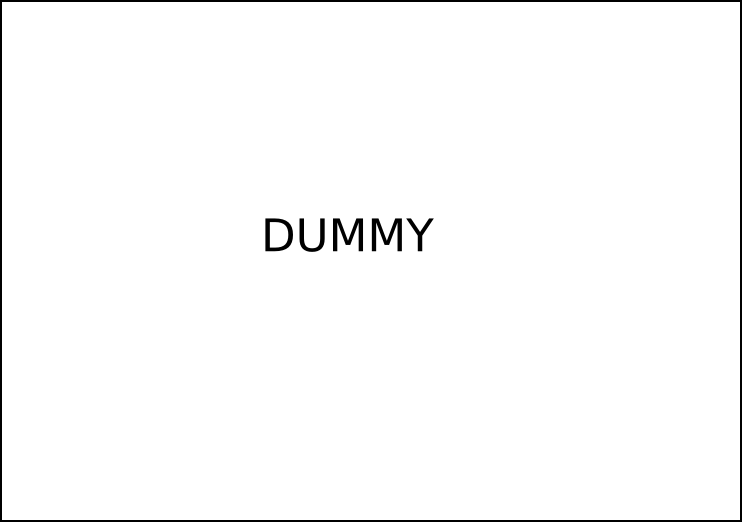
\includegraphics[width=0.8\textwidth]{Images/dummy.png}
    \caption{Hier der für die sechste Teilaufgabe angefertigte Graph. Exportieren Sie die Darstellung als PDF, legen sie im Unterordner \code{Images} ab und ändern den Befehl oben entsprechend}
\end{figure}

\section{Unsicherheiten}
Diskutieren Sie hier die Unsicherheiten des Versuchs: $\operatorname{u}(T_{20})$, $\operatorname{u}(m_F)$, ...

\section{Federkonstante und Masse der Feder}
Bitte geben Sie hier Ihre Ergebnisse für Federkonstante und Masse aus der Regression an. Bitte denken Sie auch an die Angabe der zugehörigen Messunsicherheiten.

Zum Beispiel: \underline{\underline{$k_1=\SI{3,1415\pm0,0005}{\newton\per\meter}\;.$}}

\section{Zusammenfassung}
Hier nennen Sie kurz den Inhalt der vorherigen Abschnitte (keine neuen Erkenntnisse).

\end{document}
